\section{\textbf{Sensores Internos}}
Los sensores internos se emplean para monitorear el estado interno de un robot, es decir, su posición, velocidad, aceleración, etc., en un momento determinado. Basado en estas informaciones, el controlador decide acerca del comando de control. Dependiendo de las diferentes cantidades que miden, los sensores se denominan como de posición, velocidad, aceleración o fuerza.

\subsection{\textbf{Sensores de Posición}}
Los sensores de posición miden la posición de cada articulación, es decir, el ángulo de articulación de un robot. A partir de dichos ángulos puede encontrarse la confi guración del ejecutor fi nal, y ubicar su posición y orientación por medio de la cinemática directa, que se revisará en el capítulo 6. A continuación se explican los diferentes sensores de posición.

\addcontentsline{toc}{subsubsection}{Encoder}
\subsection*{\quad\textbf{Encoder}}
El encoder es un dispositivo óptico digital que convierte el movimiento en una secuencia de pulsos digitales. Mediante el conteo de un solo bit o la decodificación de un conjunto de bits, los pulsos pueden convertirse en medidas relativas o absolutas. De este modo, los encoders son de tipo incremental o absoluto. Además, cada tipo puede ser lineal y rotatorio a su vez.

\begin{itemize}

	\item \textbf{Incremental}: este encoder tiene una escala transparente con una retícula opaca. El tamaño del espesor de las líneas de la retícula y el del espacio entre ellas son iguales y se encuentran en el rango de micrones. De un lado, la escala se equipa con una fuente de luz y un lente de condensador. Del otro, hay celdas sensibles a la luz. La resistencia de las celdas (fotodiodos) disminuye cada vez que reciben un rayo de luz. De este modo, se genera un pulso cada vez que un rayo de luz es atravesado por la línea opaca. Este pulso se introduce en el controlador que actualiza a un contador (un registro de la distancia recorrida).
	
	\item \textbf{Absoluto}: En principio, se parece al encoder lineal incremental. La diferencia es que da un valor absoluto de la distancia recorrida en cualquier momento. Así, las posibilidades de perder los pulsos a altas velocidades son menores. La salida es digital en este caso. La escala se marca con una secuencia de tiras opacas y transparentes. Si el bloque opaco que aparece en la escala de la ilustración representa 1 (uno) y el bloque transparente 0 (cero), entonces la columna de la extrema izquierda mostrará un número binario cómo 00000, es decir, un valor decimal de 0, y la columna siguiente mostrará un número binario 00001, es decir, una valor decimal de 1.
\end{itemize}

\begin{figure}[h] % h = aquí, t = top, b = bottom, p = página separada
	\centering
	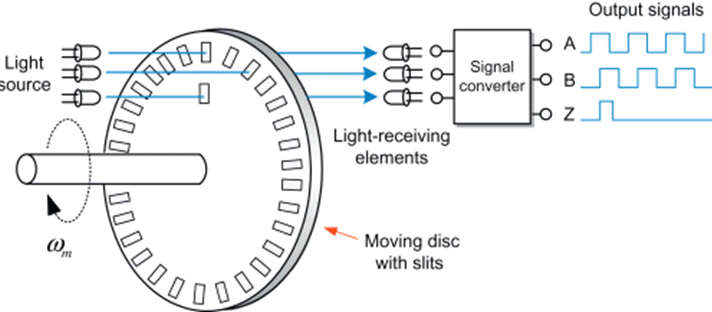
\includegraphics[width=0.6\textwidth]{encoderincr.jpg} % Ajusta el tamaño
	\caption{Encoder Incremental}
	\label{fig:ejemplo}
\end{figure}
\vspace{10cm}
\addcontentsline{toc}{subsubsection}{Potenciometro}
\subsection*{\quad\textbf{Potenciometro}}
Dispositivo de resistencia variable que expresa desplazamientos lineales o angulares en términos de voltaje, Consiste en una clavija deslizante que hace contacto con un elemento resistivo; conforme se mueve este punto de contacto, la resistencia entre el contacto deslizante y las conexiones de los extremos del dispositivo cambia en proporción al desplazamiento, x y  para potenciómetros lineales y angulares, respectivamente.

\addcontentsline{toc}{subsubsection}{LVDT}
\subsection*{\quad\textbf{LVDT}}
El transformador diferencial lineal variable (LVDT) es uno de los transductores de desplazamiento que más extensamente se usa, particularmente cuando se necesita alta precisión. Genera una señal de CA cuya magnitud se relaciona con el desplazamiento de un núcleo móvil. El concepto básico es el de un núcleo férrico que se mueve en un campo magnético, donde el campo se produce de un modo similar al campo de un transformador estándar. Existe un núcleo central, rodeado por dos bobinas secundarias idénticas y una bobina principal. Conforme el núcleo cambia su posición con respecto a las bobinas, cambia también el campo magnético y, por tanto, se modifica la amplitud de voltaje en la bobina secundaria como una función del desplazamiento del núcleo a través de un segmento considerable.

\addcontentsline{toc}{subsubsection}{Resólver}
\subsection*{\quad\textbf{Resólver}}
Los sincronizadores y resólvers son dispositivos analógicos que convierten la posición angular en señales eléctricas, a diferencia de los encoders digitales. Constan de un rotor giratorio y un estator estacionario, y requieren un convertidor analógico-digital para su procesamiento en computadoras. Los sincronizadores poseen tres devanados en el estator dispuestos a 120° en configuración "Y", lo que los hace más complejos y costosos, mientras que los resólvers tienen solo dos devanados a 90°, siendo más simples y económicos. Los resólvers modernos, especialmente los sin escobillas, utilizan un transformador para acoplar señales, eliminando el desgaste mecánico y aumentando su durabilidad. Operan en voltajes de 2V a 40V RMS y frecuencias de 400 Hz a 10 kHz, con precisiones angulares desde 5 hasta 0.5 minutos de arco. Su funcionamiento se basa en el principio del transformador rotatorio, donde la magnitud del voltaje inducido en el estator depende de la posición angular del rotor.


\subsection{\textbf{Sensores de Velocidad}}
Los sensores de velocidad realizan la medición tomando medidas de posición consecutivas a intervalos de tiempo constante, calculando la razón de cambio respecto al tiempo de los valores de posición, o lo determina en forma directa con base en diferentes principios.

\addcontentsline{toc}{subsubsection}{Todos los sensores de posición}
\subsection*{\quad\textbf{Todos los sensores de posición}}
Básicamente todos los sensores de posición, cuando se utilizan con ciertos límites de tiempo, pueden dar la velocidad, por ejemplo, el número de pulsos proporcionados por un encóder de posición incremental dividido entre el tiempo consumido en hacerlo. Sin embargo, este método impone una carga computacional sobre el controlador, que podrá estar ocupado por algunas otras operaciones.


\addcontentsline{toc}{subsubsection}{Tacómetro}
\subsection*{\quad\textbf{Tacómetro}}
Estos sensores pueden encontrar directamente la velocidad en cualquier momento y sin mucha carga computacional. Estos miden la velocidad de rotación de un elemento. Hay varios tipos de tacómetros en uso, pero un diseño sencillo se basa en la regla de Fleming, que declara que "el voltaje producido es proporcional al índice del acoplamiento inductivo". Aquí un conductor (básicamente una bobina) se sujeta al elemento rotativo que gira en un campo magnético (estator). Conforme incrementa la velocidad del eje, el voltaje producido en las terminales de las bobinas también aumenta. De otra manera, como se muestra en la figura 4.6, puede colocarse un imán sobre el eje rotativo y una bobina sobre el estator. El voltaje producido es proporcional a la velocidad de rotación del eje. Esta información se digitaliza mediante un convertidor analógico-digital y se introduce en la computadora.

\begin{figure}[h]
	\centering
	\subfloat[Perro]{%
		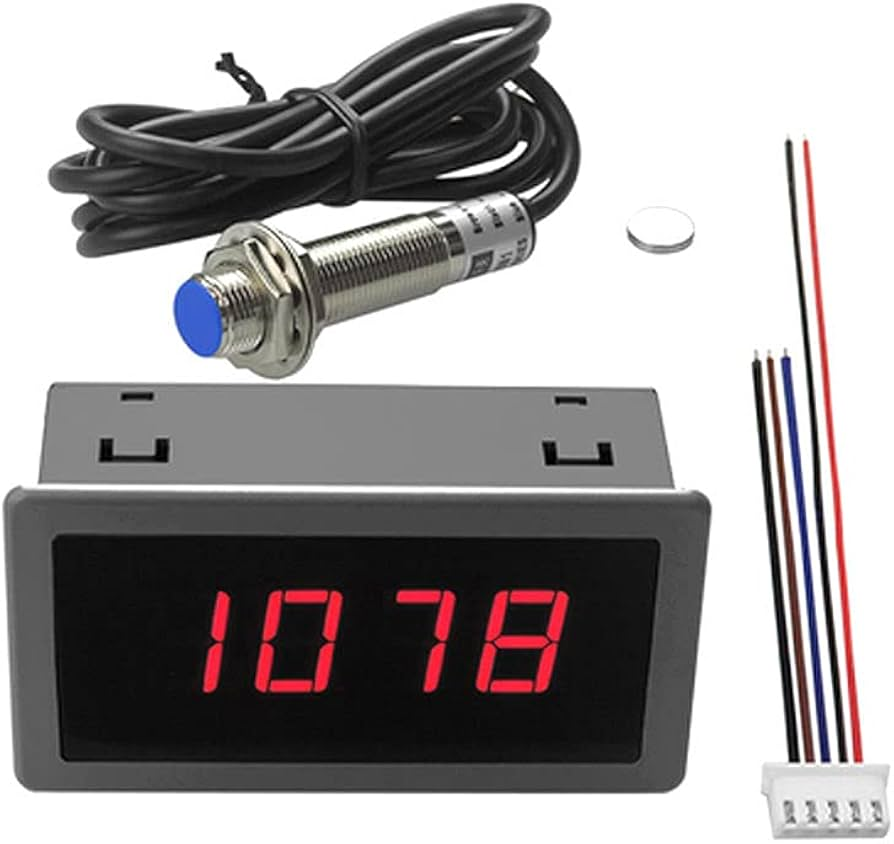
\includegraphics[width=0.2\textwidth]{tacometro.jpg}%
		\label{fig:Tacómetro Comercial}
	}
	\qquad
	\subfloat[Gato]{%
		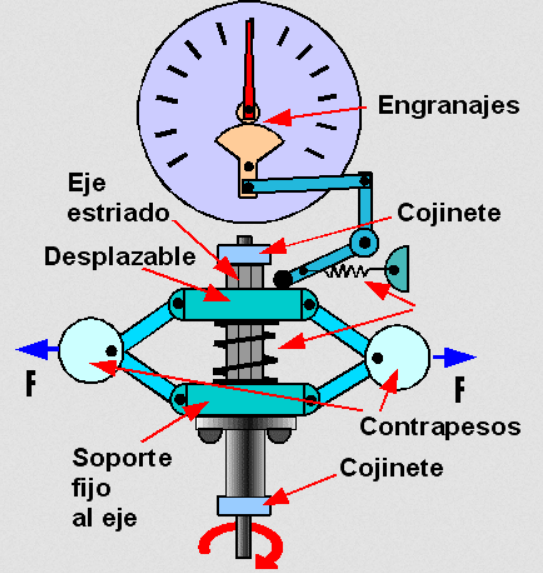
\includegraphics[width=0.2\textwidth]{tacometroDiagrama.png}%
		\label{fig:Diagrama Tacómetro}
	}
	\caption{Imagen de dos mascotas}
	\label{fig:Tacómetro}
\end{figure}

\addcontentsline{toc}{subsubsection}{Sensor de Efecto Hall}
\subsection*{\quad\textbf{Sensor de Efecto Hall}}
Otro dispositivo de medición de velocidad es el sensor de efecto Hall, cuyo principio se describe a continuación. Si una pieza plana de material conductor llamada chip Hall se sujeta a una diferencia de potencial en sus dos lados opuestos, como se indica en la figura 4.7, entonces el voltaje que se genera a través de las caras perpendiculares es cero. Pero si un campo magnético se induce en ángulos rectos al conductor, el voltaje se genera en las otras dos caras perpendiculares. Entre más alto sea el valor de campo, más lo será el nivel de voltaje. Si se utiliza un imán anular, el voltaje producido será proporcional a la velocidad de rotación del imán.


\subsection{\textbf{Sensores de Aceleración}}
De manera parecida a las mediciones de velocidad que se dan a partir de la información de los sensores de posición, pueden encontrarse las aceleraciones como la razón de cambio respecto al tiempo de las velocidades obtenidas por los sensores de velocidad o calculado a partir de las informaciones de posición. Pero ésta no es una manera efi ciente para calcular
la aceleración, puesto que impondrá una carga de trabajo pesada sobre la computadora, lo que puede reducir la velocidad de operación del sistema. Otra forma de medir la aceleración es calculando la fuerza que resulta de multiplicar masa por aceleración.

\subsection{\textbf{Sensores de Fuerza}}
Una balanza de resorte es un ejemplo de un sensor de fuerza en donde se aplica una fuerza, por ejemplo, el peso, al platillo de balanza que causa un desplazamiento, es decir, el resorte se estira. El desplazamiento es entonces una medida de la fuerza. Existen otros tipos de sensores de fuerza, por ejemplo, con base en galgas, utilizando el sensor de efecto Hall, etcétera.

\addcontentsline{toc}{subsubsection}{Galgas Extensiométricas}
\subsection*{\quad\textbf{Galgas Extensiométricas}}
El principio de este sensor es que el alargamiento de un conductor aumenta su resistencia eléctrica. La resistencia eléctrica normal para galgas es de 50-100 ohmios. El incremento de resistencia se debe a: Incremento de la longitud del conductor; y Decremento en el área del conductor. Las deformaciones ocasionan cambios en la resistencia eléctrica de las galgas, lo que se mide mediante su conexión al circuito de puente de Wheatstone como una de las cuatro resistencias. Éste es un método barato y preciso para medir deformaciones.

\addcontentsline{toc}{subsubsection}{Sensor Piezoeléctrico}
\subsection*{\quad\textbf{Sensor Piezoeléctrico}}
Un material piezoeléctrico presenta un fenómeno conocido como efecto piezoeléctrico. Este efecto señala que cuando cristales elásticos asimétricos se deforman mediante una fuerza, se desarrollará un potencial eléctrico dentro de la red cristalina deformada. Este efecto es reversible. Esto quiere decir que si se aplica un voltaje entre las superficies del cristal, éste cambiará sus dimensiones físicas. La magnitud y polaridad de las cargas inducidas son proporcionales a la magnitud y dirección de la fuerza aplicada. Los materiales piezoeléctricos son cuarzo, turmalina, sal de Rochalle y otros. El rango de fuerzas que pueden medirse usando sensores piezoeléctricos es de 1 a 20 kN y con una proporción de 2×1052×105. Estos sensores pueden usarse para medir un cambio instantáneo en la fuerza (fuerzas dinámicas).
\cite{saha2014robotica}
\pagebreak





